\documentclass[border=15pt]{standalone}
\usepackage{tikz,amsmath,amssymb}
\usetikzlibrary{arrows.meta}
\usepackage{tikzcats}   % 原生保留 tikzcats

% ========== 画布级字号 ==========
\newcommand{\bigf}{\fontsize{26}{32}\selectfont}
\newcommand{\smallf}{\fontsize{22}{28}\selectfont}
\newcommand{\tinyf}{\fontsize{20}{26}\selectfont}

% ========== 配色方案 ==========
% 左侧自然室内背景配色
\definecolor{wallCol}{RGB}{248, 245, 238}      % 雅致奶杏白墙面
\definecolor{floorCol}{RGB}{225, 198, 168}     % 暖色原木地板
\definecolor{skirtCol}{RGB}{198, 170, 140}     % 踢脚线
\definecolor{rugCol}{RGB}{190, 218, 210}       % 莫兰迪薄荷绿地毯
\definecolor{rugBorder}{RGB}{155, 190, 180}
\definecolor{windowSky}{RGB}{205, 235, 248}    % 窗外明净天空
\definecolor{windowFrame}{RGB}{160, 110, 70}   % 窗框原木色
\definecolor{artFrame}{RGB}{130, 85, 50}       % 壁画框深木色

% 右侧语义分割掩码配色 (经典学术规范：高对比度纯色色块)
\definecolor{maskBg}{RGB}{32, 36, 48}          % 背景类别 (Background)
\definecolor{maskCat}{RGB}{235, 65, 55}        % 猫咪目标类 (Cat: 鲜亮珊瑚红)

% ========== 宏定义：与 \cat 完全几何同构的纯色语义分割掩码 ==========
\def\catmask#1{
\scope[scale=3]
    % 尾巴
    \draw[line width=15pt, #1, cap=round] (0,-2.3) .. controls +(-2,0) and (-2,-1.3) .. (-1.5,-1);
    \draw[line width=15pt, #1, cap=round] (-1.5,-1) .. controls +(0.9,0.4) and (-1.1,0.1) .. (-1.5,0);
    % 身体轮廓
    \fill[#1] (0.5,-2) circle (0.5);
    \fill[#1] (-0.5,-2) circle (0.5);
    \fill[#1, rounded corners=50pt] (-0.5,-2.5) rectangle (0.5,-0.3);
    \fill[#1] (0.4,-2.5) .. controls (0.3,-0.5) and (-0.3,-0.5) .. (-0.4,-2.5);
    % 前爪与后腿
    \fill[#1] (0.4,-1.6) ellipse (0.2 and 0.9);
    \fill[#1, rounded corners=10pt] (0.6,-2.52) rectangle (0.2,-2.25);
    \fill[#1] (-0.4,-1.6) ellipse (0.2 and 0.9);
    \fill[#1, rounded corners=10pt] (-0.6,-2.52) rectangle (-0.2,-2.25);
    % 头部与耳朵
    \fill[#1] (0,0) circle (0.65);
    \fill[rounded corners=8pt, #1] (0,0.5) -- (-0.6,1) -- (-0.7,0.8) -- (-0.6,0) -- cycle;
    \fill[rounded corners=8pt, #1] (0,0.5) -- (0.6,1) -- (0.7,0.8) -- (0.6,0) -- cycle;
    % 下巴与脸颊
    \fill[#1] (0,-0.5) ellipse (0.25 and 0.2);
    % 胡须 (与掩码颜色完全一致)
    \draw[line width=1.5pt, #1, cap=round] (0.15,-0.34) .. controls (0.3,-0.31) and (0.6,-0.32) .. (0.8,-0.39);
    \draw[line width=1.5pt, #1, cap=round] (0.15,-0.39) .. controls (0.3,-0.36) and (0.55,-0.42) .. (0.75,-0.49);
    \draw[line width=1.5pt, #1, cap=round] (-0.15,-0.34) .. controls (-0.3,-0.31) and (-0.6,-0.32) .. (-0.8,-0.39);
    \draw[line width=1.5pt, #1, cap=round] (-0.15,-0.39) .. controls (-0.3,-0.36) and (-0.55,-0.42) .. (-0.75,-0.49);
\endscope
}

\begin{document}
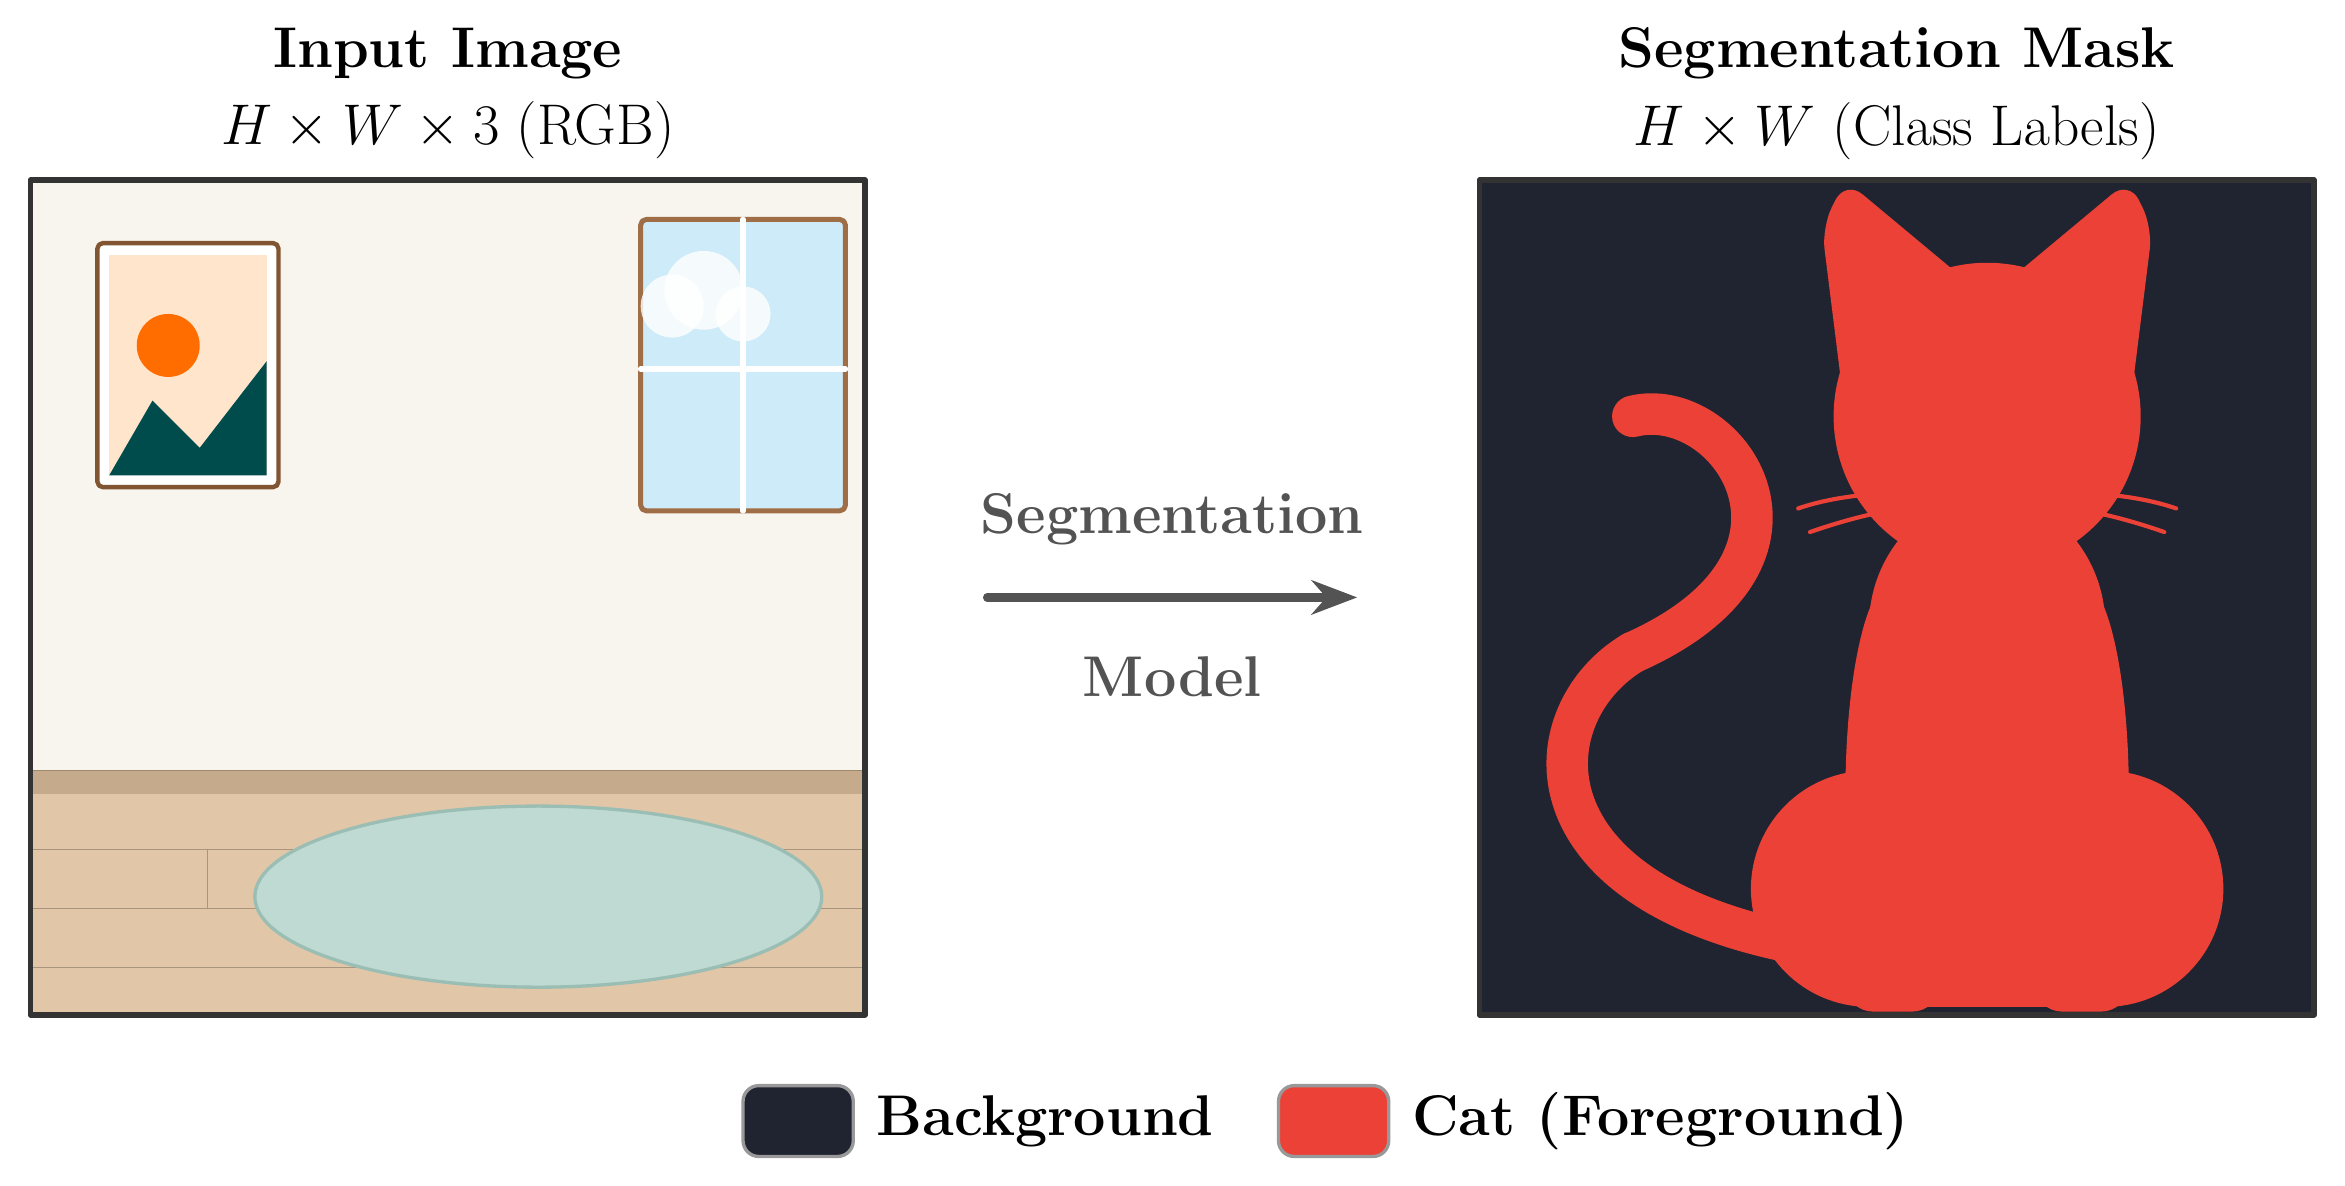
\begin{tikzpicture}[
    font=\bigf, line join=round, line cap=round,
    every node/.style={inner sep=0pt, outer sep=0pt, align=center},
    arr/.style={->, >=Stealth, line width=3pt, color=darkgray!90}
  ]

  % 1. 左侧：输入图像 (Input Image, 10.6 x 10.6 正方形)
  \begin{scope}
    % 标题
    \node[font=\smallf\bfseries] at (4.65, 19.5) {Input Image\\{\tinyf\normalfont \(H\times W\times 3\) (RGB)}};

    % 裁剪到正方形框 (-0.65, 7.8) 到 (9.95, 18.4)
    \clip (-0.65, 7.8) rectangle (9.95, 18.4);

    % --- 背景：温馨雅致的现代室内 ---
    % 上半部：奶杏色温暖墙面
    \fill[wallCol] (-0.65, 10.9) rectangle (9.95, 18.4);

    % 墙面挂画 (极简日落风景画)
    \draw[artFrame, fill=white, line width=1.6pt, rounded corners=2pt] (0.2, 14.5) rectangle (2.5, 17.6);
    \fill[orange!20] (0.35, 14.65) rectangle (2.35, 17.45);
    \fill[orange!85!red] (1.1, 16.3) circle (0.4);
    \fill[teal!60!black] (0.35, 14.65) -- (0.9, 15.6) -- (1.5, 15.0) -- (2.35, 16.1) -- (2.35, 14.65) -- cycle;

    % 墙面阳光大窗 (右侧)
    \draw[windowFrame, fill=windowSky, line width=1.8pt, rounded corners=2pt] (7.1, 14.2) rectangle (9.7, 17.9);
    % 窗外白云
    \fill[white, opacity=0.8] (7.5, 16.8) circle (0.4);
    \fill[white, opacity=0.8] (7.9, 17.0) circle (0.5);
    \fill[white, opacity=0.8] (8.4, 16.7) circle (0.35);
    % 白色十字窗格
    \draw[white, line width=2pt] (8.4, 14.2) -- (8.4, 17.9);
    \draw[white, line width=2pt] (7.1, 16.0) -- (9.7, 16.0);

    % 踢脚线
    \fill[skirtCol] (-0.65, 10.6) rectangle (9.95, 10.9);
    \draw[skirtCol!80!black, line width=.6pt] (-0.65, 10.9) -- (9.95, 10.9);

    % 下半部：实木地板与木纹接缝
    \fill[floorCol] (-0.65, 7.8) rectangle (9.95, 10.6);
    \foreach \fy in {8.4, 9.15, 9.9} {
      \draw[floorCol!75!black, line width=.5pt] (-0.65, \fy) -- (9.95, \fy);
    }
    \draw[floorCol!75!black, line width=.5pt] (1.6, 9.15) -- (1.6, 9.9);
    \draw[floorCol!75!black, line width=.5pt] (6.2, 9.15) -- (6.2, 9.9);
    \draw[floorCol!75!black, line width=.5pt] (3.6, 8.4) -- (3.6, 9.15);
    \draw[floorCol!75!black, line width=.5pt] (8.1, 8.4) -- (8.1, 9.15);

    % 柔软圆形猫咪地毯
    \fill[rugCol, draw=rugBorder, line width=1.2pt] (5.8, 9.3) ellipse (3.6 and 1.15);

    % 前景：猫咪主体 (调用原生 tikzcats 宏)
    \begin{scope}[shift={(5.8, 15.4)}]
      \cat
    \end{scope}
  \end{scope}
  \draw[black!80, line width=2pt] (-0.65, 7.8) rectangle (9.95, 18.4);

  % 2. 中间：直接连接的大箭头与模型标注
  \draw[arr] (11.5, 13.1) -- (16.2, 13.1);
  \node[font=\smallf\bfseries, text=darkgray!90] at (13.85, 14.1) {Segmentation};
  \node[font=\smallf\bfseries, text=darkgray!90] at (13.85, 12.1) {Model};

  % 3. 右侧：分割掩码 (Segmentation Mask, 纯净高清矢量无杂线)
  \begin{scope}[shift={(18.4, 0)}]
    % 标题
    \node[font=\smallf\bfseries] at (4.65, 19.5) {Segmentation Mask\\{\tinyf\normalfont \(H\times W\) (Class Labels)}};

    % 裁剪到与左侧绝对一致的正方形框 (-0.65, 7.8) 到 (9.95, 18.4)
    \clip (-0.65, 7.8) rectangle (9.95, 18.4);

    % 背景：完全纯净的深色背景掩码 (无杂乱网格线)
    \fill[maskBg] (-0.65, 7.8) rectangle (9.95, 18.4);

    % 前景：几何严格对齐的纯红猫咪掩码 (像素级精确重合)
    \begin{scope}[shift={(5.8, 15.4)}]
      \catmask{maskCat}
    \end{scope}
  \end{scope}
  \draw[black!80, line width=2pt] ({18.4-0.65}, 7.8) rectangle ({18.4+9.95}, 18.4);

  % 4. 底部：简洁居中的类别图例 (无公式，干净清爽)
  \begin{scope}[shift={(8.4, 6.0)}]
    \fill[maskBg, draw=black!40, line width=1.2pt, rounded corners=2mm] (0, 0) rectangle ++(1.4, 0.9);
    \node[font=\smallf\bfseries, anchor=west] at (1.7, 0.45) {Background};

    \fill[maskCat, draw=black!40, line width=1.2pt, rounded corners=2mm] (6.8, 0) rectangle ++(1.4, 0.9);
    \node[font=\smallf\bfseries, anchor=west] at (8.5, 0.45) {Cat (Foreground)};
  \end{scope}

\end{tikzpicture}
\end{document}